% not fixed

\chapter{TINJAUAN PUSTAKA}
\label{chap:tinjauanpustaka}

% Ubah bagian-bagian berikut dengan isi dari tinjauan pustaka

\section{Penelitian Terdahulu}
\label{sec:penelitianterdahulu}
% state of the art

% not good
\subsection{Penelitian Berkaitan dengan \textit{Smart Whiteboard}}
\label{subsec:penelitianterkaitsmartwhiteboard}
Kellerman et al. \citep*{kellerman2018smart} mencoba untuk menyediakan suatu cara alternatif dan terjangkau pada papan tulis atau slides agar bisa mendapat interaksi lebih dari murid serta untuk meningkatkan efisiensi dari pengajaran. Pada penelitiannya, peneliti membuat sebuah papan tulis interaktif menggunakan Nintendo Wii \textit{Remote} dan \textit{PC Suite}. \textit{Software Suite} yang dikembangkan memungkinkan tampilan PC apapun dapat digunakan sebagai papan tulis interaktif. Sistem yang dibangun memiliki fungsi yang diperlukan untuk menciptakan sarana pembelajaran yang lebih baik dan lebih berteknologi, serta memberi pengguna dan siswa alat tambahan untuk menunjang Pendidikan interaktif. \textit{PC Suite} dibuat seramah mungkin sehingga dapat digunakan dengan mudah pada komputer standar. \par

% is good
\subsection{Penelitian Berkaitan dengan \textit{Word Detection}}
\label{subsec:penelitianterkaitworddetection}
Arun et al. \citep*{arun2019handwritten} menyajikan pendekatan sederhana untuk segmentasi huruf kata tulisan tangan menggunakan pendekatan bounding box dan pendekatan berbasis pixel. Segmentasi huruf tulisan tangan merupakan proses yang menantang karena gaya penulisan yang bervariasi. Kata-kata tulisan tangan yang tidak bersentuhan disegmentasikan dengan pendekatan bounding box dan kata-kata tulisan tangan yang bersentuhan disegmentasi menggunakan pendekatan pixel. Paper ini mencapai tingkat segmentasi hingga 94.45\% dan tingkat pengenalan 85.89\% dengan skema training dan testing 50-50\%. \par

% not good
\subsection{Penelitian Berkaitan dengan YOLO \textit{Object Detection}}
\label{subsec:penelitianterkaityolo}
Karlina dan Indarti \citep*{karlina2020pengenalan} membuat pengenalan objek Makanan cepat saji dari \textit{video} dan \textit{real time webcam} menggunakan metode \textit{deep learning. You Only Look Once (YOLO)} merupakan model \textit{deep learning} yang digunakan untuk pengenalan objek. Jumlah data yang digunakan terdiri dari 468 gambar yang terdiri dari 3 jenis Makanan cepat saji. Nilai avg loss pada model akhir yang dibangun yaitu 4.6\%, nilai validasi mAP 100\%, serta akurasi akhir berkisar antara 63\% sampai 100\%. \par


% % Contoh input gambar
% \begin{figure}[ht]
%   \centering

%   % Ubah dengan nama file gambar dan ukuran yang akan digunakan
%   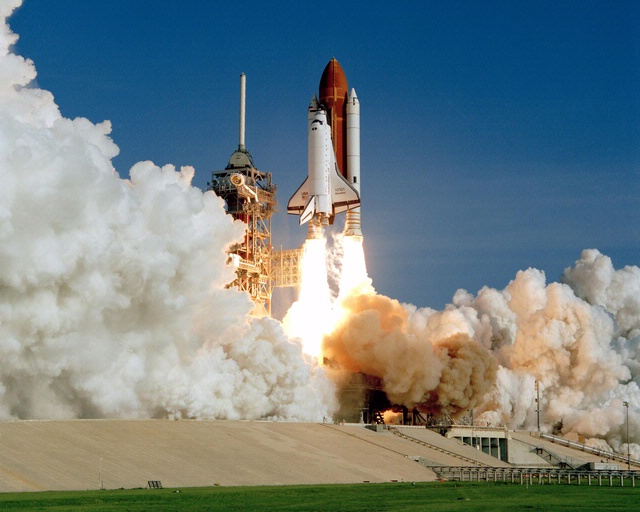
\includegraphics[scale=0.35]{gambar/roketluarangkasa.jpg}

%   % Ubah dengan keterangan gambar yang diinginkan
%   \caption{Peluncuran roket luar angkasa \emph{Discovery} \citep{roketluarangkasa}.}
%   \label{fig:roketluarangkasa}
% \end{figure}

% Roket luar angkasa merupakan \lipsum[1]

% \emph{Discovery}, Gambar \ref{fig:roketluarangkasa}, merupakan \lipsum[2]

% Per Teori Penunjang dibuat section baru

\section{\textit{Deep Learning}}
\label{sec:deeplearning}
\textit{Deep learning} (DL) merupakan cabang dari \textit{machine learning} yang didasarkan pada \textit{artificial neural network}.DL memungkinkan model komputasi dari beberapa lapisan pemrosesan untuk mempelajari dan mewakili data dengan berbagai tingkat abstraksi. \textit{Deep learning} merupakan metode yang memiliki implementasi sangat banyak mencakup \textit{Neural Networks, hierarchical probabilistic models, unsupervised} dan \textit{supervised learning} \citep*{voulodimos2018deep}. \textit{Deep Learning} dirancang untuk dapat terus mengolah data dan menganalisa data tersebut seperti dalam mengambil keputusan. Adapun dalam \textit{Deep Learning, training} suatu data dipengaruhi oleh banyaknya jumlah layer dan jumlah neuron. Artinya, semakin banyak layer atau neuron yang digunakan maka akan semakin lama proses yang dilakukan, hal ini disebabkan oleh tingkat kompleksitas yang semakin besar juga. \par

% not good
\section{Convolutional Neural Network (CNN)}
\label{sec:convolutionalneuralnetwork}
CNN merupakan algoritma \textit{deep learning}yang mampu mengambil masukan berupa gambar, menetapkan prioritas untuk berbagai aspek/objek dalam gambar dan mampu membedakan satu sama lain. Tahapan \textit{pre-processing} yang dibutuhkan CNN lebih sedikit jika dibandingkan dengan algoritma klasifikasi lainnya \citep*{towardsDS}. \textit{Convolutional Neural Network (CNN)} itu sendiri juga merupakan pengembangan dari \textit{Multilayer Percepton (MLP)} yang didesain untuk mengolah data dua dimensi. CNN termasuk dalam jenis \textit{Deep Neural Network} karena kedalaman jaringan yang tinggidan banyak diaplikasikan pada data citra \citep*{putra2016klasifikasi}.\par
Secara sederhana, CNN memiliki beberapa jenis \textit{neural layers} yang masing-masing memiliki peranannya masing-masing \citep*{voulodimos2018deep}. Adapun secara sederhana CNN terdiri dari 3 jenis utama \textit{neural layers} yaitu: \par
\begin{enumerate}[nolistsep]
    \item \textit{Convolutional Layers}
    \item \textit{Pooling Layers}
    \item \textit{Fully Connected Layers}
\end{enumerate}
\indent Secara umum, cara kerja CNN hampir serupa pada MLP, hanya saja dalam CNN setiap neuron dipresentasikan dalam bentuk dua dimensi. Adapun cara kerja dari suatu MLP sederhana yaitu MLP semula memiliki sejumlah \textit{layer} dengan masing-masing layer memiliki sejumlah \textit{neuron}. MLP menerima masukan data dalam bentuk satu dimensi, kemudian mempropagasikan data tersebut pada jaringan sehingga didapat hasil keluaran. Setiap hubungan antar \textit{neuron} pada dua \textit{layer} yang bersebelahan memiliki parameter bobot satu dimensi yang menentukan kualitas mode. Disetiap data input pada layer dilakukan operasi linear dengan nilai bobot yang ada, kemudian hasil komputasi akan ditransformasi menggunakan operasi non linear yang disebut sebagai fungsi aktivasi. \par


\section{Confusion Matrix}
\label{sec:confusionmatrix}

\section{Mean Average Precision (mAP)}
\label{sec:meanaverageprecision}

\section{Object Detection}
\label{sec:objectdetection}
\textit{Object Detection} adalah sebuah proses untuk mendeteksi suatu instance objek semantik dari kelas tertentu (seperti bentuk, huruf, pesawat, angka, dan lain lain) dalam sebuah gambar atau video. Pendekatan umum dari  \textit{frameworks} deteksi objek mencakupi pembuatan set besar yang diklasifikasikan secara sekuel menggunakan fitur CNN \citep*{voulodimos2018deep}. \par

% keknya gaperlu ??
% \section{Word Segmentation}
% \label{sec:wordsegmentation}
% Pengenalan tulisan tangan merupakan Teknik untuk menginterpretasikan tulisan tangan kedalam bentuk digital. Proses pengenalan tulisan tangan dapat diperoleh dengan 2 cara yaitu dengan mengonversi otomatis karakter pada saat ditulis pada layar sentuh dengan pena digital dan cara lain yaitu dengan melakukan pengambilan gambar serta pemrosesan gambar pada suatu teks yang ingin dikenali [8]. Pada proses segmentasi huruf, mulanya dokumen gambar disegmentasi kedalam baris-baris teks. Kemudian, algoritma segmentasi huruf diterapkan pada satu baris teks tersebut. Pada satu baris teks tersebut, secara umum proses segmentasi huruf konvensional menjalankan algoritma yang terdiri dari 2 tahapan yaitu: ekstraksi kandidat huruf berdasarkan pemisah huruf dan dilanjut dengan klasifikasi kandidat huruf \citep*{ryu2015word}.

\section{You Only Look Once (YOLO)}
\label{sec:yolo}
YOLO merupakan salah satu arsitektur dari CNN yang dioptimasi untuk mendeteksi objek pada gambar. Arsitektur YOLO sangat cepat apabila dibandingkan dengan arsitektur pengenalan objek lainnya . YOLO melakukan proses pengenalan objek berbasis CNN dalam sebuah kotak yang disebut \textit{anchor} yang dipusatkan pada 13x13 \textit{grid cell} dalam sebuah gambar. Artinya, ukuran gambar diubah (dikurangi) menjadi 416x416 terlepas dari ukuran asli dari gambar yang ingin di proses \textit{train or detect}. Artinya, jika terdapat perbedaan besar dalam rasio gambar yang diproses \textit{train}, maka akan terjadi distorsi serius pada objek ketika dilakukan proses penyesuaian ukuran\citep*{jeong2018image}. \par

% Kemudian menjadi persamaan seperti pada persamaan \ref{eq:hukumpertamanewton}.

% % Contoh pembuatan persamaan
% \begin{equation}
%   \label{eq:hukumpertamanewton}
%   \sum \mathbf{F} = 0\; \Leftrightarrow\; \frac{\mathrm{d} \mathbf{v} }{\mathrm{d}t} = 0.
% \end{equation}
